\vspace{-3mm}
\section{晶圆级 GEMM}\label{sec:gemm}
\vspace{-1mm}

本节介绍 \gemm：一种可扩展到超大规模网格架构的分布式 GEMM。

\vspace{-3mm}
\subsection{分布式 GEMM 的 PLMR 符合性}
\vspace{-1mm}

\begin{figure}
    \centering
    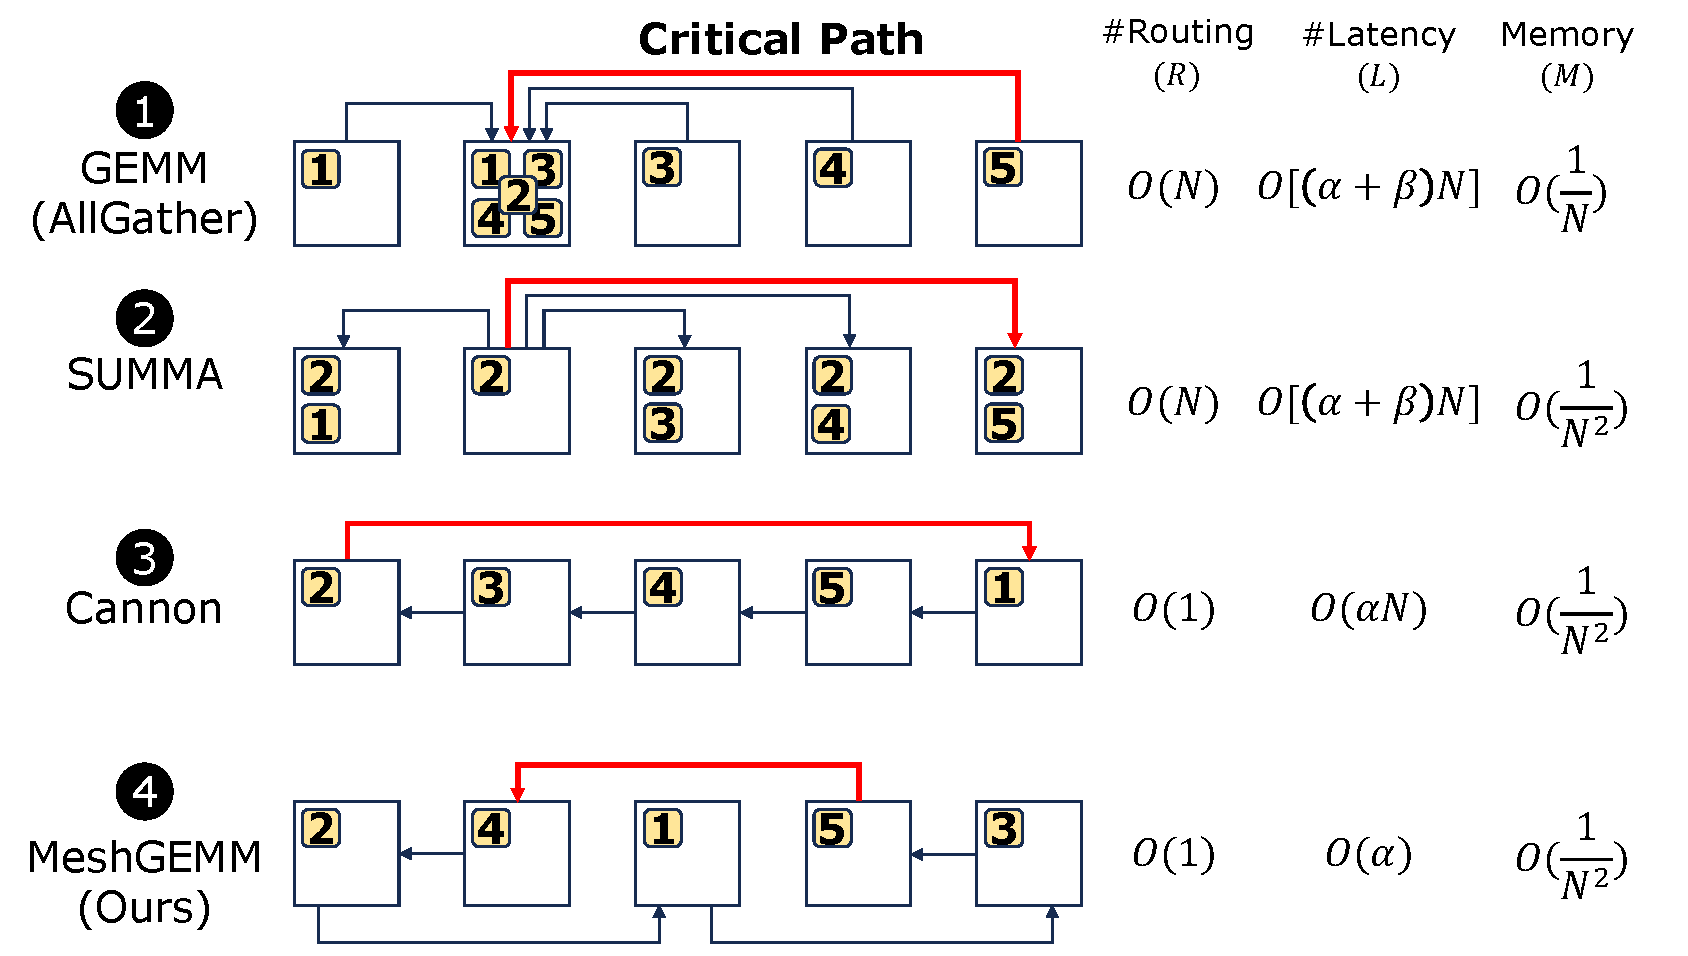
\includegraphics[width=1\linewidth]{imgs/gemm-analysis.pdf}
    \vspace{-3mm}
    \caption{分布式 GEMM 的 PLMR 符合性}
    \vspace{-3mm}
    \label{fig:distributed-gemm-analysis}
\end{figure}

为了找出适用于 PLMR 设备、能够扩展的分布式 GEMM，我们定义以下指标：
（i）\emph{单核路由路径数}：每个核心使用的路由路径数量；路径越少，越符合 R 属性。
（ii）\emph{关键路径延迟}：每一步传输子矩阵的所有通信路径中的最大延迟，即图~\ref{fig:distributed-gemm-analysis} 中的红线；延迟越低，越符合 L 属性。
（iii）\emph{单核内存}：每个核心所需内存；用量越低，越符合 M 属性。

下面分析现有分布式 GEMM 方法，并说明 \gemm 如何满足这些指标。

\begin{enumerate}[label=(\arabic*),leftmargin=0.5cm,noitemsep,topsep=0pt]
\item \textbf{基于 Allgather 的 GEMM} 常用于 GPU 和 TPU pod 上的分布式 GEMM~\cite{google2023efficiently,tensorrt-llm,megatron}。每一步的关键通信路径，是某个核心从最远核心收集数据的路径，如图~\ref{fig:distributed-gemm-analysis} 的 \circled{1} 中红线所示；完成 allgather 共需 $N$ 步。每个核心要为同一行和同一列中的邻居建立 $N$ 条路由路径（违反 R）。R 约束迫使系统经由中间核心逐步传输子矩阵，使关键路径产生 $O[(\alpha+\beta)N]$ 的通信延迟（违反 L）；膨胀的工作缓冲区还使单核使用 $O(1/N)$ 内存（违反 M）。

\item \textbf{SUMMA} 是 Cerebras 晶圆级引擎默认采用的分布式 GEMM~\cite{cerebrasgemm}。每一步的关键通信路径，是一个核心沿列或行把数据广播到最远核心的路径，如图~\ref{fig:distributed-gemm-analysis} 的 \circled{2} 中红线所示。与 \circled{1} 中的 allgather 相同，每个核心建立 $N$ 条路由路径（违反 R），每一步关键路径的延迟为 $O[(\alpha+\beta)N]$（违反 L）。尽管 SUMMA 的内存用量优于 allgather，只需要与本地划分子矩阵等大的工作集，但峰值内存仍会翻倍。

\item \textbf{Cannon} 是针对网格优化的分布式 GEMM~\cite{cannon}，广泛用于超级计算机与分布式集群。每一步的关键通信路径，是头部核心把数据发送到尾部核心的路径，如图~\ref{fig:distributed-gemm-analysis} 的 \circled{3} 所示。每个中间核心在 2D 环面中与两个邻居通信，并将子矩阵从头部传递到尾部，因此只需 $O(1)$ 条通信路径，内存用量也达到最优的 $O(1/N^2)$。

值得注意的是，Cannon 的单核路由路径数为常数，因此可以为邻居通信与关键路径分配静态路由规则。每一步中，子矩阵都可通过中间核心从头部直接传到尾部，不像基于 allgather 的 GEMM 或 SUMMA 那样必须逐步传递消息。因此，关键路径只产生单跳延迟 $\alpha$，没有额外的单次路由开销 $\beta$。但是关键路径仍跨越 $N$ 跳，所以延迟依然为 $O(\alpha N)$，如 \circled{3} 的红线所示，违反 L。

\item \textbf{MeshGEMM（本文方法）} 是一种符合 PLMR 模型的分布式 GEMM。我们把每一步的关键通信路径称为“两跳传输”，如图~\ref{fig:distributed-gemm-analysis} 的 \circled{4} 中红线所示；它显著短于其他方法。每个核心与两个相距两跳的邻居通信，并穿过一个单跳邻居的通信路径（后文将证明，该方法可以扩展到更大的网格架构）。与 Cannon 相同，这一设计只需要 $O(1)$ 条单核通信路径，内存用量也达到最优的 $O(1/N^2)$。关键在于，它把关键路径恒定限制为 2 跳，复杂度为 $O(\alpha)$，因而是这些方法中唯一能满足 L 属性的方案。
\end{enumerate}

\vspace{-0.2cm}
\subsection{设计直觉与可扩展性分析}

我们的设计分为两个阶段：（i）通过 GEMM 的循环移位过程保证算法正确性；（ii）再用交错排列把关键路径延迟限制为常数。循环移位与交错排列共同形成\textbf{两跳传输}通信路径；我们还证明，在这一循环上，两跳是满足 L 属性所需的最短距离。

\begin{figure}[t!]
    \centering
    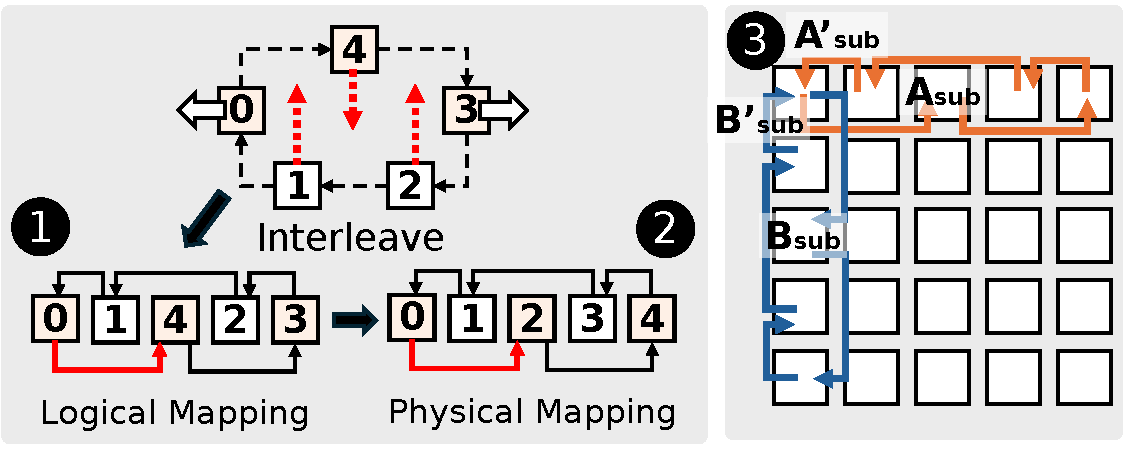
\includegraphics[width=1\linewidth]{imgs/gemm_intuition.pdf}
    \caption{设计直觉与可扩展性分析。}
    \label{fig:gemm_intuition}
\end{figure}

\mypar{循环移位} 循环移位把通信限制在两个邻居之间，并尽量降低内存用量，使 \gemm 满足 M 与 R 属性。它以类似 Cannon~\cite{cannon} 的推理保证 GEMM 结果正确。如图~\ref{fig:distributed-gemm-analysis} 的 \circled{3} 所示，一个由 5 个核心构成的逻辑环被展开到物理通信映射中，其中存在一条从头部核心到尾部核心的关键路径。

\begin{algorithm}[t]
    \caption{$\textbf{INTERLEAVE}$}
    \label{alg:interleave}
    \SetKwFunction{assert}{assert}
    \SetKw{ret}{返回}
    \SetKw{int}{Int}
    \LinesNumbered
    \KwIn{index, N}
    \KwOut{send\_index, recv\_index}

    \eIf{\textnormal{index} \textnormal{\textbf{ mod }} \textnormal{2 == 0}}{
        recv\_index = \texttt{Max}(index - 2, 0)\;
        send\_index = \texttt{Min}(index + 2, N - 1)\;
    }{
        recv\_index = \texttt{Min}(index + 2, N - 1)\;
        send\_index = \texttt{Max}(index - 2, 0)\;
    }
    \textbf{若} \textnormal{index == 0} \textbf{则} recv\_index = 1\;
    \If{\textnormal{index == N - 1}}{
        \textbf{若} N \textbf{ mod } 2 == 0 \textbf{则}
            recv\_index = N - 2\;
        \textbf{否则}
            send\_index = N - 2\;
    }
    \ret send\_index, recv\_index\;
\end{algorithm}


\mypar{交错排列} 对于展开后的通信方案，我们希望进一步缩短关键路径，从而满足 L 属性。核心思路是引入 INTERLEAVE 操作，寻找从逻辑位置到物理位置的映射关系，其定义见算法~\ref{alg:interleave}。如图~\ref{fig:gemm_intuition} 的 \circled{1} 所示，\gemm 先把核心 1 插入核心 0 与核心 4 之间，再把核心 2 插入核心 4 与核心 3 之间，形成逻辑映射；随后调用 INTERLEAVE，得到发送目标邻居与接收来源邻居的索引，最终得到图~\ref{fig:gemm_intuition} 中 \circled{2} 所示的、经过置换但等价的通信方案。例如，总共有 5 个核心（$N=5$），物理核心 2（index=2）便向物理核心 4（send\_index=4）发送数据，并从物理核心 0（recv\_index=0）接收数据。图~\ref{fig:distributed-gemm-analysis} 与图~\ref{fig:gemm_intuition} 以 5 个核心为例，而算法~\ref{alg:interleave} 表明，\gemm 的两跳通信模式可以推广到任意 $N\geq3$ 的网格架构。

\mypar{可扩展性分析} 我们可以证明，INTERLEAVE 产生的两跳距离无法进一步缩短。证明依赖序列排列的基本性质：若试图构造一个循环序列，并要求每个数字与相邻数字恰好相差一跳，就会遇到数学上的不可能。把数字想象成直线上的点即可理解：相邻数字虽然可以连接，但序列的两个端点不可能在组成环的同时，仍与各自邻居都保持一跳之差。

以上讨论基于一维数组，但可以自然推广到二维网格，因为一维数组分别对应网格中对称的 $X$ 轴和 $Y$ 轴。

\vspace{-0.3cm}
\subsection{\gemm 算法}\label{subsec:meshgemm}

\gemm 的关键步骤如下。

\begin{enumerate}[label=(\arabic*),leftmargin=0.5cm,noitemsep,topsep=0pt]
\item \textbf{初始化：} 考虑 $C=A\times B$。\gemm 沿两个维度把 $A$ 与 $B$ 划分为 $A_{sub}$ 和 $B_{sub}$ tile，形成分布在各核心上的 $N\times N$ 个 tile。每个核心接收一个 $A_{sub}$ tile 和一个 $B_{sub}$ tile。随后，\gemm 使用 INTERLEAVE 初始化每个核心的邻居位置。

\item \textbf{对齐：} 每个核心与邻居对齐输入子矩阵，保证分布式系统中的每个核心在开始矩阵乘法时都持有正确的操作数。

\item \textbf{计算--移位循环：} 每个核心执行一个包含 $N$ 步通信与计算的计算--移位循环。每一步中，每个核心都计算其对应的部分和 $C_{sub}=A_{sub}\times B_{sub}+C_{sub}$；同时沿 $X$ 轴移位 $A_{sub}$、沿 $Y$ 轴移位 $B_{sub}$，得到下一步计算所需的新 $A'_{sub}$ 与 $B'_{sub}$，如图~\ref{fig:gemm_intuition} 的 \circled{3} 所示。执行 $N$ 步后，返回累积的 $C_{sub}$。
\end{enumerate}

\vspace{-0.3cm}
\subsection{实现细节}

\mypar{处理非方形网格} 对于非方形网格 $N_h\times N_w$（$N_h\neq N_w$），可以在逻辑上把 $A$、$B$ 矩阵划分到 $N_{lcm}\times N_{lcm}$ 个核心，其中 $N_{lcm}$ 是 $N_h$ 与 $N_w$ 的最小公倍数。

\mypar{转置式分布式 GEMM} 上述算法还可用于计算 $C=A\times B^T$，即图~\ref{fig:prefill-partition} 中用来避免在网格上转置 $B$ 的 dist-GEMM-T。计算前无需对齐，只需沿 $Y$ 轴对右矩阵 $B$ 执行 $N$ 步两跳计算--移位。每一步移位后，每个核心计算 $C_{\text{sub}}=A_{\text{sub}}\times B_{\text{sub}}$，随后沿 $X$ 轴对 $C_{\text{sub}}$ 执行 ReduceAdd。经过 $N$ 步即可得到最终矩阵 $C$。
